\phantomsection
%\addcontentsline{toc}{chapter}{Introduzione}
\chapter{GreenCloud Simulator Overview}
\markboth{GreenCloud Simulator Overview}{}
% [titolo ridotto se non ci dovesse stare] {titolo completo}

\begin{citazione}

\end{citazione}
\newpage

\section{Selection of GreenCloud} 
Based on the comparisons made among the different analyzed simulators, each of them has its strengths and weaknesses. However, for the needs required in the study addressed by this thesis work, it is essential to prioritize aspects related to the energy consumption of the computing center and the accuracy of simulations. From the conducted comparisons, it is evident that \emph{GreenCloud} is the simulator that accurately considers these aspects as it is built on top of \emph{NS2} simulator and fully implements the \emph{TCP/IP} protocol. Moreover, \emph{GreenCloud} offers its users a set of features related to the simulation and to the energy consumption management. In particular, it is possible to choose between several pre-implemented Data Center architectures and energy models as well as to customize them. Furthermore \emph{GreenCloud} provides various workload scheduling and power saving models, allowing programmers to implement new ones. Despite \emph{GreenCloud} simulation times tend to be high, for the purposes of this study it is reasonable to prioritize granularity over performance. Therefore, the study will continue using \emph{GreenCloud} as the reference tool for the simulations to be conducted. The following sections provide a description of various aspects of \emph{GreenCloud} based on the work by \emph{Kliazovich et al} \cite{kliazovich2012greencloud}.


\section{Available Data Center architectures}
As mentioned in the previous section, \emph{GreenCloud} provides several Data Centers architectures. The implemented architectures consist of various components, described as follows:
\begin{itemize}
    \item \textbf{Servers: } single core nodes with a fixed processing power limit expressed in \emph{MIPS} (million instructions per second) or \emph{FLOPS} (floating point operations per second) that are responsible for task execution. These components are organized in racks and the architecture includes the presence of a Top-of-Rack switch that connects them to the access layer of the architecture;
    \item \textbf{Switches and links: } they implement the interconnection between the Servers in the Data Center. The type and the quality of these devices influences the transmission rate, anyway the costs of such devices need to be taken into account. Switches usually support either 1 \emph{GE (Gigabit Ethernet)} or 10 \emph{GE} as transmission rates, while links usually support 10 \emph{Mb/s}, 100 \emph{Mb/s}, and 1 \emph{Gb/s} as transmission rates;
    \item \textbf{Workloads: } the representation of tasks to be executed that consist of two components, computational and communicational. The computational part specifies the required amount of computing resources, measured in \emph{MIPS} or \emph{FLOPS}, and the duration of resource allocation. On the other hand, the communicational component of the workload entails the quantity and dimensions of data transfers essential before, during, and after the workload execution.
\end{itemize}
The following subsections provide an overview of the available Data Center architectures within the \emph{GreenCloud} simulator. Since, as mentioned in the previous chapter, this simulator is based on \emph{NS2}, it is possible to customize the \emph{Data Center} architecture. 

\subsubsection{Two-tier Data Center architecture}
Two-tier architecture is shown in figure \ref{fig:greencloud_twotier}. This architecture consists of an \emph{Access Network} layer where rack switches group several computing Servers through 1 \emph{GE} links and a \emph{Core Network} layer where L3 switches provide full mesh connectivity through 10 \emph{GE} links. This type of architecture supports up to 5500 nodes.
\begin{figure}[h]
    \centering
    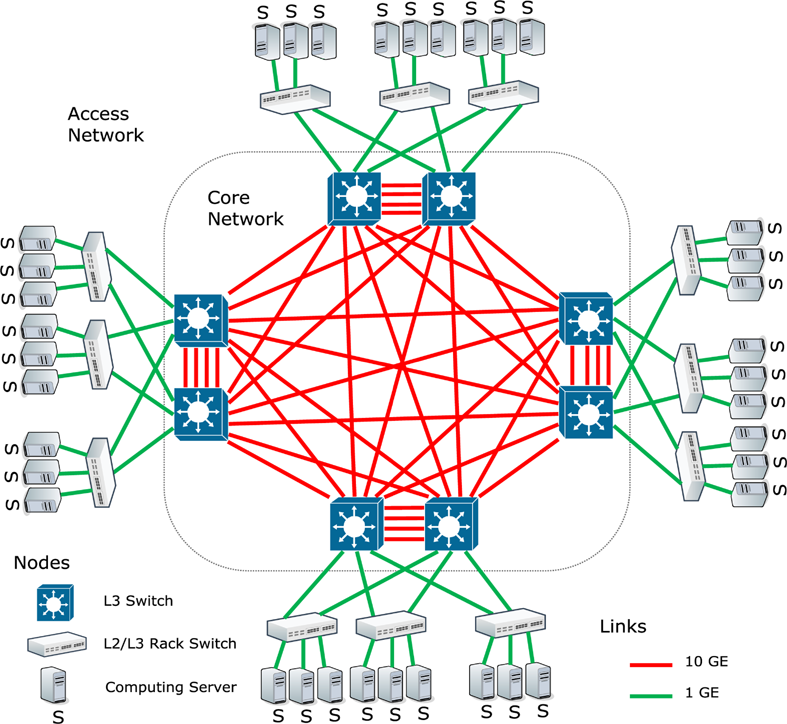
\includegraphics[width=0.5\textwidth]{chapters/images/greencloud_twotier.png}
    \caption{GreenCloud two-tier architecture}
    \label{fig:greencloud_twotier}
\end{figure}

\subsubsection{Three-tier Data Center architecture}
Three-tier architecture is shown in figure \ref{fig:greencloud_threetier}. This architecture consists of an \emph{Access Network} layer where rack switches group several computing Servers through 1 \emph{GE} links, an \emph{Aggregation Network} and a \emph{Core Network} where L3 switches provide full mesh connectivity through 10 \emph{GE} links. This type of architecture is the most commonly used nowadays.

\begin{figure}[h]
    \centering
    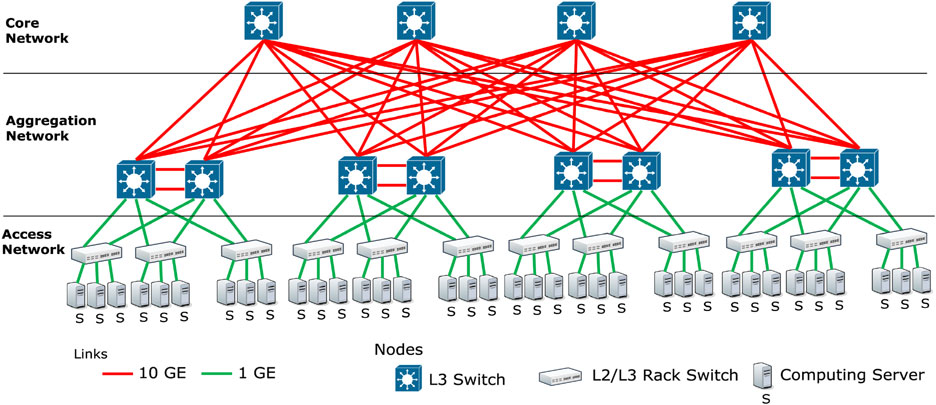
\includegraphics[width=0.7\textwidth]{chapters/images/greencloud_threetier.png}
    \caption{GreenCloud three-tier architecture}
    \label{fig:greencloud_threetier}
\end{figure}

\subsubsection{Three-tier high-speed Data Center architecture}
Three-tier high-speed architecture is shown in figure \ref{fig:greencloud_threetierhs}. This architecture is analogous to the three-tier architecture except it employs 100 \emph{GE} links in the \emph{Aggregation Network} and \emph{Core Network} instead of 10 \emph{GE} ones. Moreover, it consists of only two L3 Switches in the \emph{Core Network} instead of 4.
\begin{figure}[h]
    \centering
    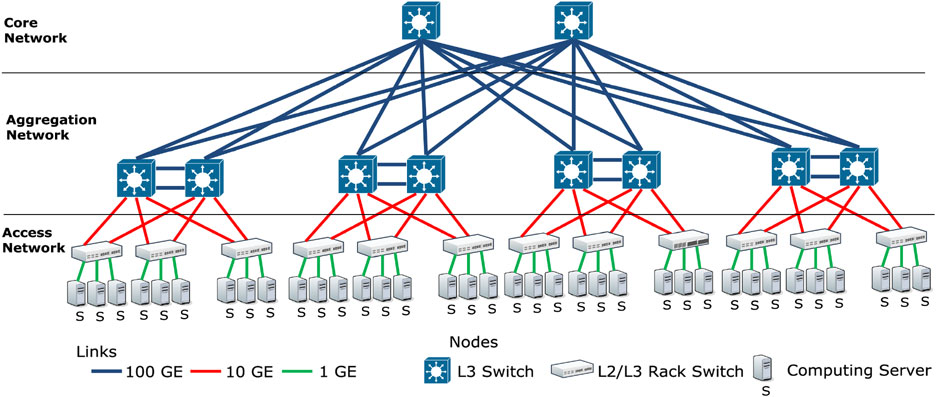
\includegraphics[width=0.7\textwidth]{chapters/images/greencloud_threetierhs.png}
    \caption{GreenCloud three-tier high-speed architecture}
    \label{fig:greencloud_threetierhs}
\end{figure}

\section{Available power saving models}
Two power saving models are available within the \emph{GreenCloud} simulator, namely \emph{Dynamic Voltage and Frequency Scaling (DVFS)} which makes the energy consumption of servers proportional to their operating frequency and \emph{Dynamic Network Shutdown (DNS)} which places idle servers into a sleep mode. The power savings achieved through these techniques are not negligible. According to \cite{kliazovich2012greencloud} the use of \emph{DVFS} results in a power savings of 4\%, the use of \emph{DNS} leads to a savings of 63\%, and the combined use of both techniques results in a savings of 65\%. It is evident that the most significant contribution comes from the utilization of \emph{DNS}, as an active server consumes a considerable amount of energy that does not scale with the operating frequency.

\section{Energy model of servers, switches, memory and disks}
Since \emph{GreenCloud} aims to be suitable for energy management, the authors provided the energy models related to the components of the \emph{Data Center} architecture. The following subsections present the energy models described in \cite{kliazovich2012greencloud} for each described component.
\subsubsection{Servers}
Assuming that \(f\) is the operating frequency of the CPU, \(P_fixed\) is the fixed energy consumption that does not scale with \(f\) and \(P_f\) is the CPU-dependent energy consumption, the total energy consumption of a server is calculated as follows (equation \ref{eq:server_energy}):
\begin{equation} \label{eq:server_energy}
    P_{server} = P_{fixed} + P_f \cdot f^3
\end{equation}
\subsubsection{Switches}
The power consumption model for switches is illustrated in \cite{makaratzis2018energy} and is described by the following equation (equation \ref{eq:switch_energy}):
\begin{equation} \label{eq:switch_energy}
    P_{switch} = P_{chassis} + n_cP_{linecard} + \sum_{r=1}^{R} n^r_pP^r_pu^r_p,
\end{equation}
where \(P_{chassis}\) is the energy consumed by the switch hardware, \(n_c\) is the number of line cards, \(n_p^r\) is the number of ports running at rate \(r\),  \(P_{linecard}\) is the energy consumed by a linecard, \(P_p^r\) is the energy consumed by a port running at rate \(r\) and \(u_p^r\) represents a port utilization, defined as follows (equation \ref{eq:port_utilization}):
\begin{equation} \label{eq:port_utilization}
    u_p = \frac{1}{T} \int_{t}^{t+T} \frac{B_p(t)}{C_p} dt = \frac{1}{T\cdot C_p} \int_{t}^{t+T} B_p(t) dt,
\end{equation}
where \(B_p(t)\) is an instantaneous throughput at the port's link at the time \(t\), \(C_p\) is the link capacity, and \(T\) is a measurement interval. 
\subsubsection{Memory and disks}
\emph{GreenCloud} implements a simple energy model for memory and disks as it allows to choose between the idle and the maximum power of these components resulting respectively in the minimum and the maximum consumption. 

\section{Workload scheduling algorithms} 
The choice of the scheduling algorithm significantly affects the energy consumption of the data center. As previously mentioned, \emph{GreenCloud} provides various scheduling algorithms and, due to its open-source nature, allows developers to create new ones. This section provides an overview of the algorithms available within the simulator and conducts a comparison among them.
\subsection{Algorithms description}

\subsection{Algorithms comparison}
    
